\section{Variables for VBF BDT} \label{app:vbf-variables}

% TODO: once variables in framework, switch these to official plots

This appendix contains distributions for variables considered for the BDT to define the VBF signal region. All histograms in this appendix are normalized such that their integral is unity. Preselection and a 4-jet requirement has been applied.

\begin{figure}[htbp]
    \centering
    \subfloat{
      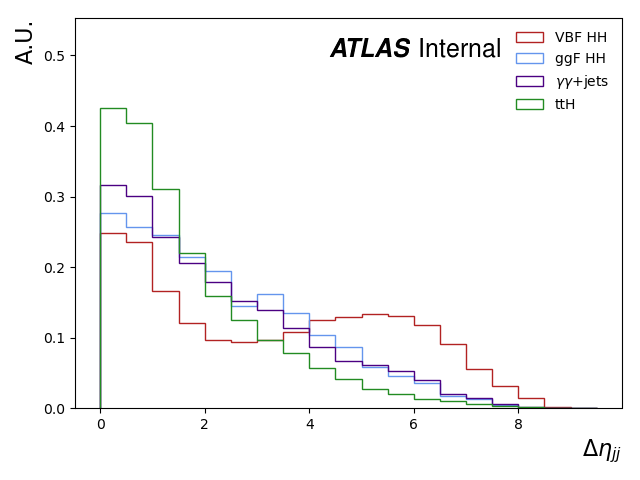
\includegraphics[width=0.48\textwidth]{appendices/vbf-variables/jj_deta.png}
    }
    \subfloat{
      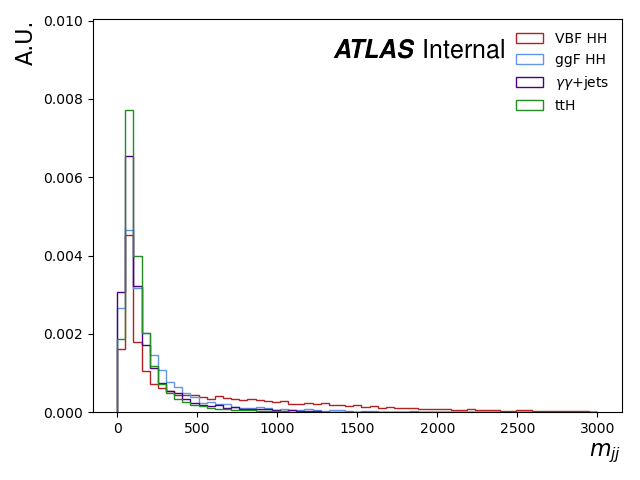
\includegraphics[width= 0.48\textwidth]{appendices/vbf-variables/mjj.png}
    }

    \subfloat{
        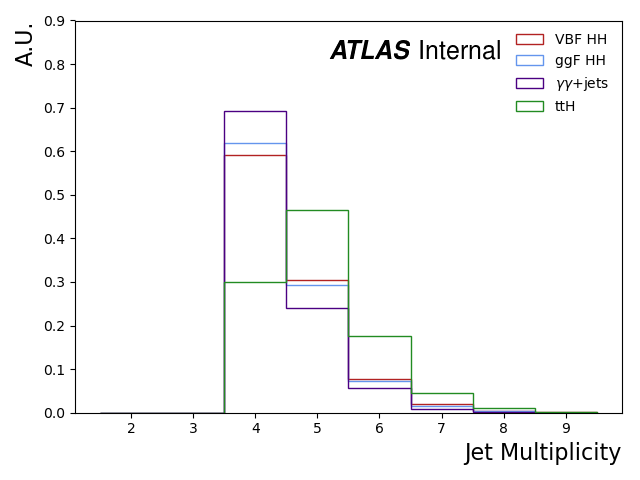
\includegraphics[width=0.48\textwidth]{appendices/vbf-variables/n_jet.png}
      }
      \subfloat{
        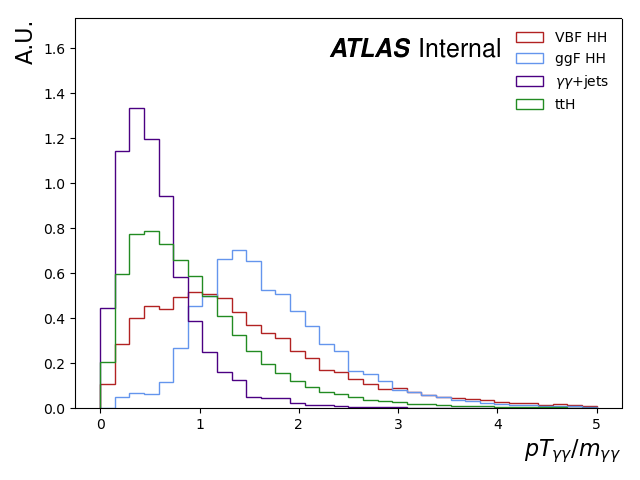
\includegraphics[width= 0.48\textwidth]{appendices/vbf-variables/ptyy_myy_ratio.png}
      }

    \subfloat{
        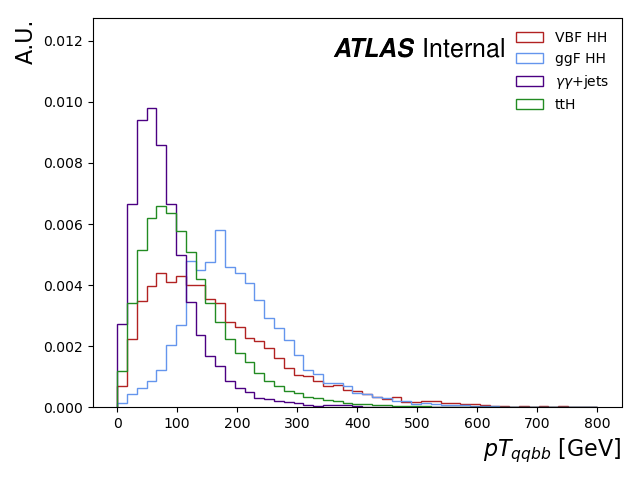
\includegraphics[width= 0.48\textwidth]{appendices/vbf-variables/pt_qqbb.png}
    }    
    \subfloat{
        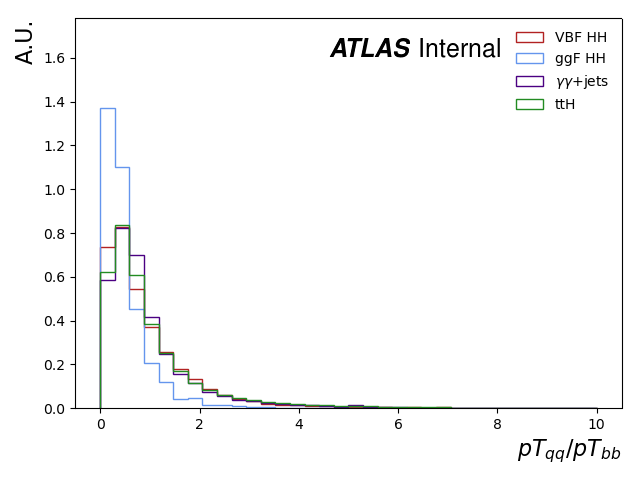
\includegraphics[width= 0.48\textwidth]{appendices/vbf-variables/pt_qq_bb_ratio.png}
    }  

    \caption{Distributions of variables for targeting VBF HH production considered for use the VBF BDT}
    \label{fig:vbf-focused-variables}
\end{figure}


\begin{figure}[htbp]
    \centering
    \subfloat{
      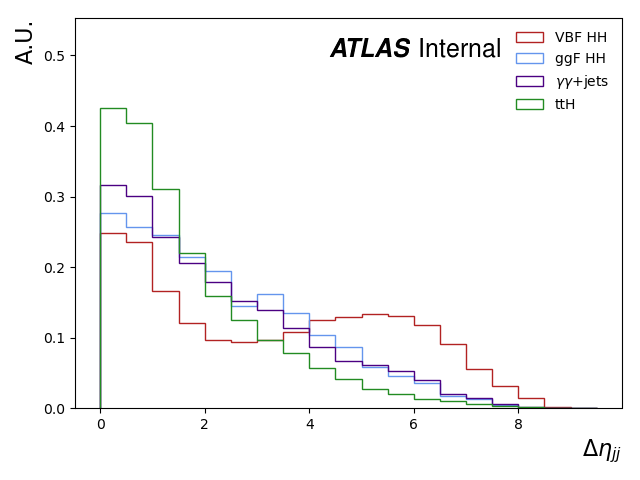
\includegraphics[width=0.48\textwidth]{appendices/vbf-variables/jj_deta.png}
    }
    \subfloat{
      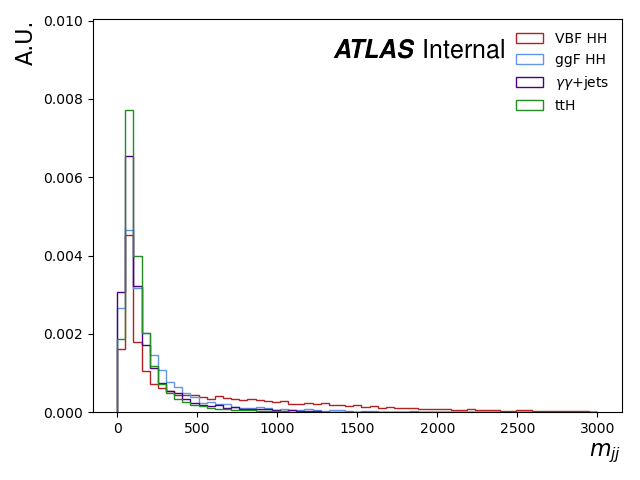
\includegraphics[width= 0.48\textwidth]{appendices/vbf-variables/mjj.png}
    }

    \subfloat{
        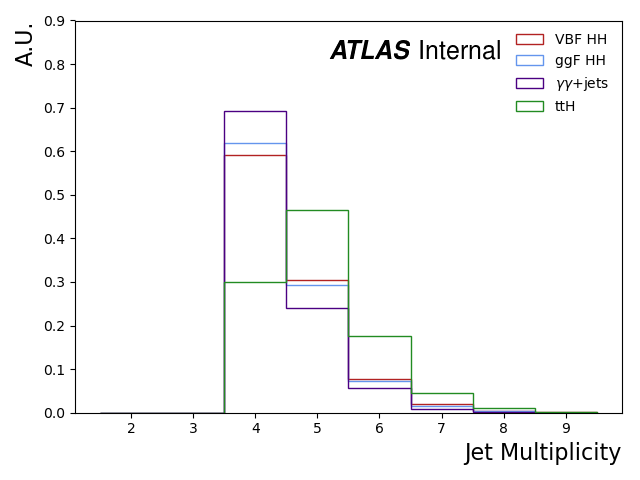
\includegraphics[width=0.48\textwidth]{appendices/vbf-variables/n_jet.png}
      }
      \subfloat{
        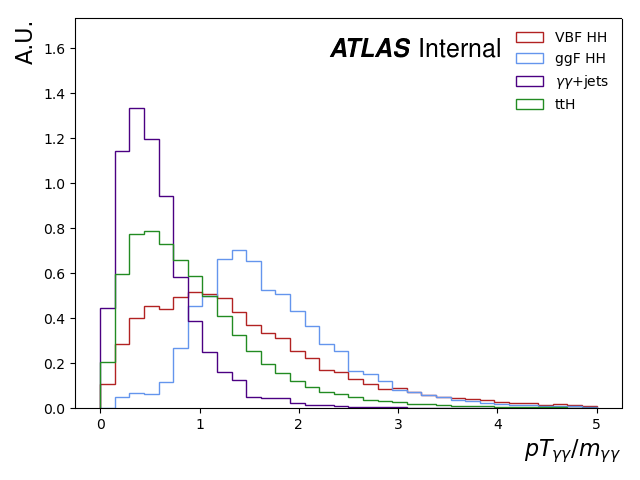
\includegraphics[width= 0.48\textwidth]{appendices/vbf-variables/ptyy_myy_ratio.png}
      }

    \subfloat{
        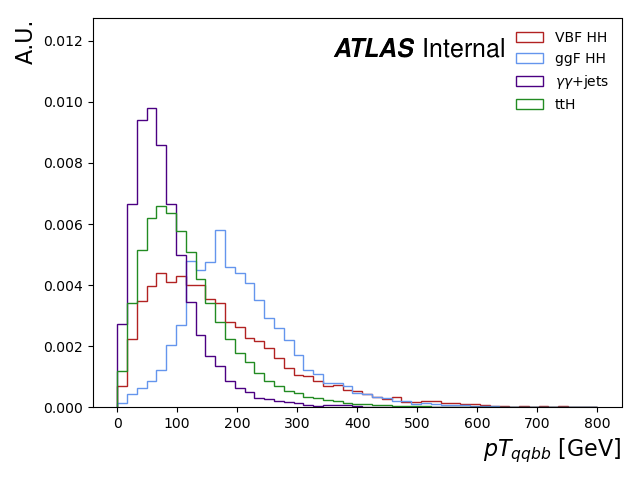
\includegraphics[width= 0.48\textwidth]{appendices/vbf-variables/pt_qqbb.png}
    }    
    \subfloat{
        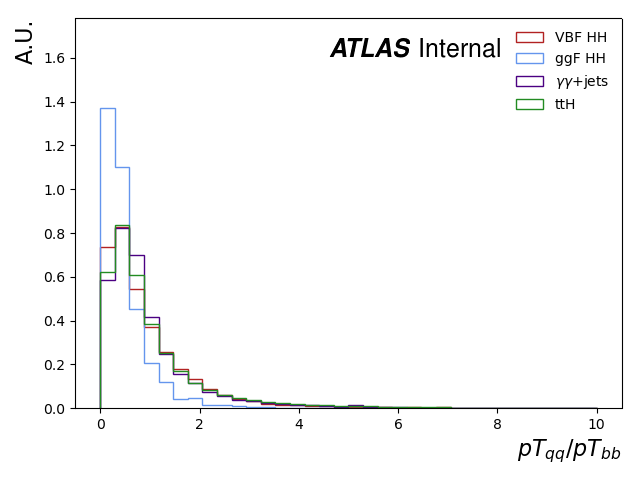
\includegraphics[width= 0.48\textwidth]{appendices/vbf-variables/pt_qq_bb_ratio.png}
    }  

    \caption{Distributions of variables for targeting VBF HH production considered for use the VBF BDT}
    \label{fig:vbf-focused-variables}
\end{figure}

\begin{figure}[htbp]
    \centering
    \subfloat{
      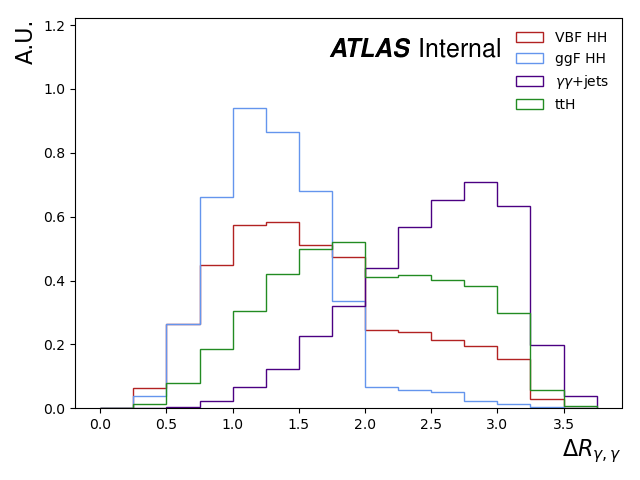
\includegraphics[width=0.48\textwidth]{appendices/vbf-variables/dR_yy.png}
    }
    \subfloat{
      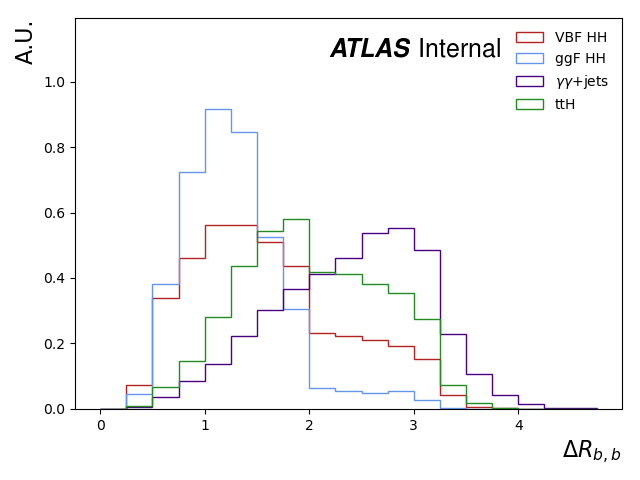
\includegraphics[width= 0.48\textwidth]{appendices/vbf-variables/dR_bb.png}
    }

    \subfloat{
        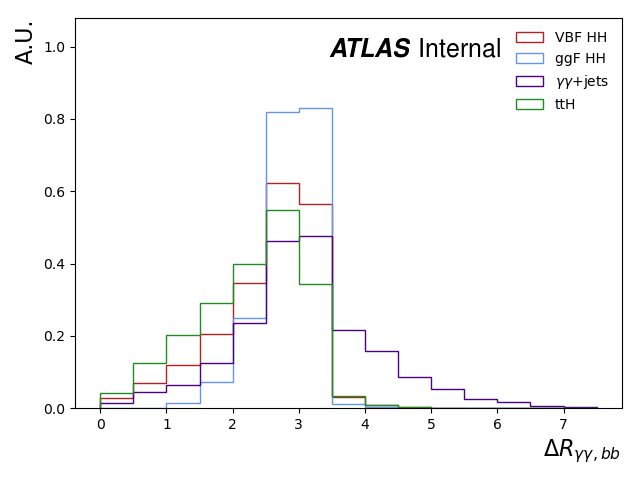
\includegraphics[width=0.48\textwidth]{appendices/vbf-variables/dR_yybb.png}
      }
      \subfloat{
        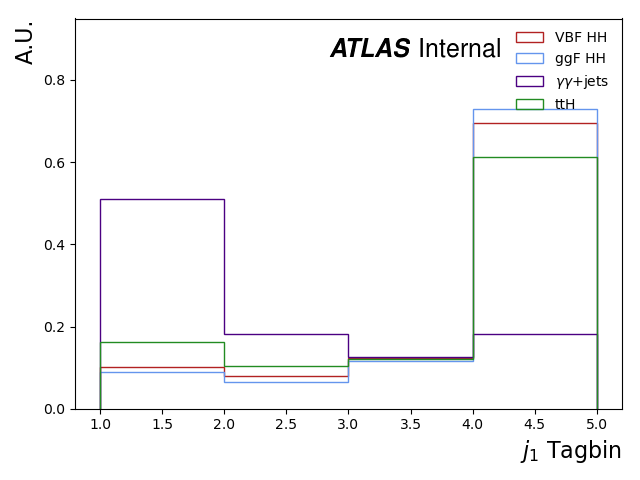
\includegraphics[width= 0.48\textwidth]{appendices/vbf-variables/j1_tagbin.png}
      }

    \subfloat{
        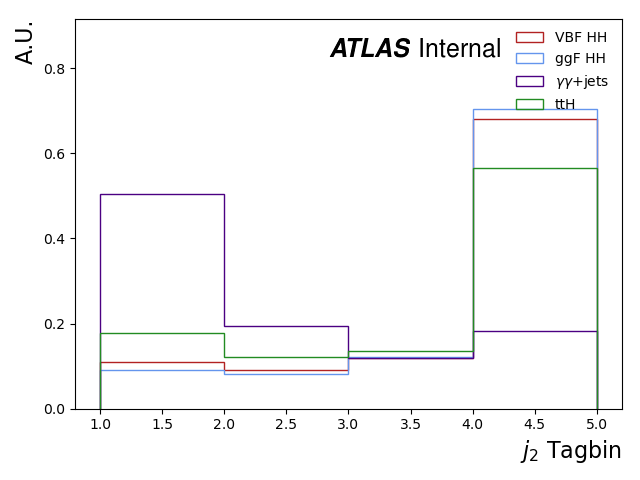
\includegraphics[width= 0.48\textwidth]{appendices/vbf-variables/j2_tagbin.png}
    }    

    \caption{Distributions of variables for suppressing the $\gamma\gamma$ background considered for use the VBF BDT}
    \label{fig:yy-focused-variables}
\end{figure}

% TODO: add w-mass variables

\begin{figure}[htbp]
    \centering
    \subfloat{
      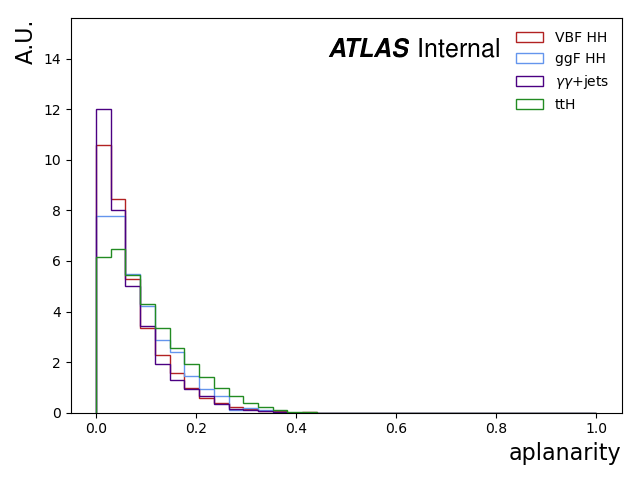
\includegraphics[width=0.48\textwidth]{appendices/vbf-variables/aplanority.png}
    }
    \subfloat{
      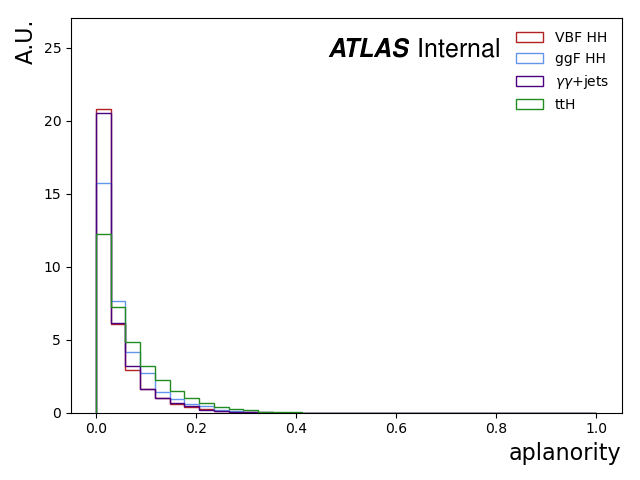
\includegraphics[width= 0.48\textwidth]{appendices/vbf-variables/aplanarity.png}
    }

    \subfloat{
        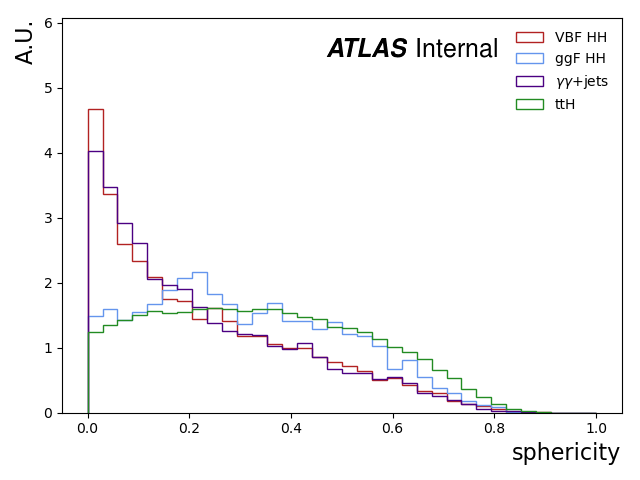
\includegraphics[width=0.48\textwidth]{appendices/vbf-variables/sphericity.png}
      }
      \subfloat{
        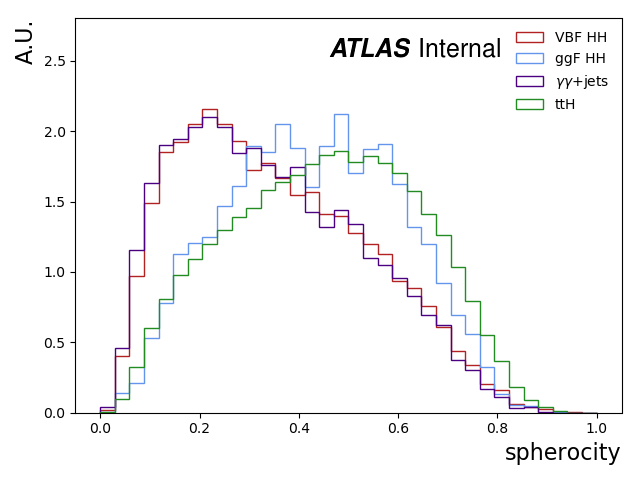
\includegraphics[width= 0.48\textwidth]{appendices/vbf-variables/spherocity.png}
      }

    \subfloat{
        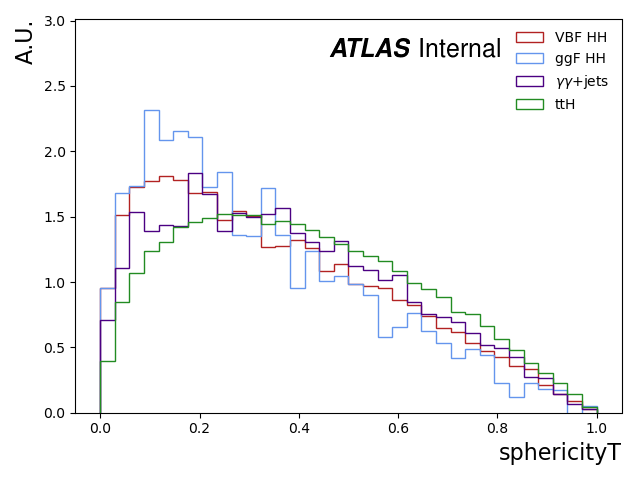
\includegraphics[width= 0.48\textwidth]{appendices/vbf-variables/sphericityT.png}
    }   
    \subfloat{
        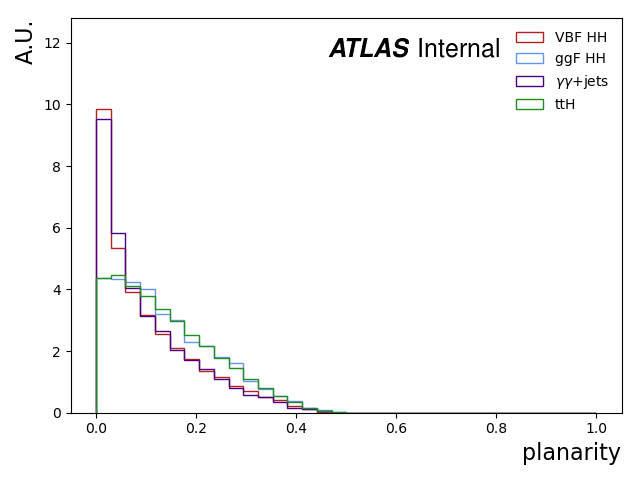
\includegraphics[width= 0.48\textwidth]{appendices/vbf-variables/planarity.png}
    }  

     

    \caption{Distributions of event shape for suppressing the $ttH$ background considered for use the VBF BDT}
    \label{fig:yy-focused-variables}
\end{figure}
\begin{figure}[htbp]\ContinuedFloat
    \subfloat{
        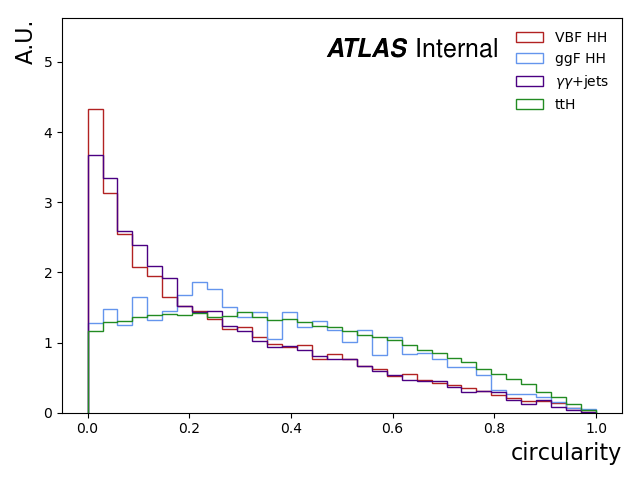
\includegraphics[width= 0.48\textwidth]{appendices/vbf-variables/circularity.png}
    }  
    \subfloat{
        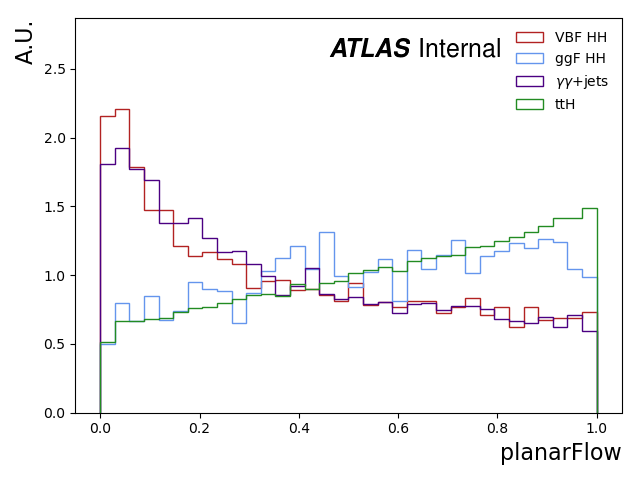
\includegraphics[width= 0.48\textwidth]{appendices/vbf-variables/planarFlow.png}
    }       
        
    \caption{Distributions of event shape for suppressing the $ttH$ background considered for use the VBF BDT}
    \label{fig:yy-focused-variables}
\end{figure}
